Przedstawiony algorytm negocjacji został zaczerpnięty z~pracy \emph{Production sequencing as negotiation}~\cite{wooldridge1996production}. W~ninejszej pracy, autorzy proponują rozwiązanie problemu planowania sekwencji pracy w~fabryce, zamieniając problem na zadanie negocjacji w~systemie agentowym.

Pomysł zamiany problemu na zadanie negocjacji opiera się na założeniu, że fabrykę można podzielić na kilka komórek. Z~każdą komórką związana jest funkcja kosztu, która opisuje pewien koszt wytworzenia elementu. Koszt produkcji związany jest z~zarówno wykonaniem samego elementu, jak i~zależy od wcześniej wykonywanego elementu. Przykładowo, stacja lakiernicza, która ostatnio pracowała z~czerwonym lakierem, w~celu wykonania zielonego elementu, musi zmienić lakier, wyczyścić dysze oraz wykonać szereg innych prac, z~którymi można utożsamić pewien koszt.

W~systemie agentowym, negocjacja sekwencji polega na rozmowie pomiędzy agentami, reprezentującymi poszczególne komórki fabryki, podczas której każdy z~agentów próbuje zmaksymalizować swoją funkcję użyteczności, czyli \emph{de facto} zminimalizować swój koszt. Koszt związany z~samą produkcją jest stały dla każdej zadanej sekwencji, dlatego też minimalizowany będzie koszt zmian typu produktu.

Podejście agentowe ma wiele zalet. W~pierwszej kolejności, takie rozwiązanie jest modularne, co pozwala na łatwe rozszerzanie, dołączanie i~wyłączanie komponentów. Rozbicie problemu na podproblemy, pozwala znacząco uprościć problem optymalizacji oraz potencjalnie przyspieszyć proces szukania rozwiązania, poprzez zrównoleglenie obliczeń.

\begin{figure}
    \centering
    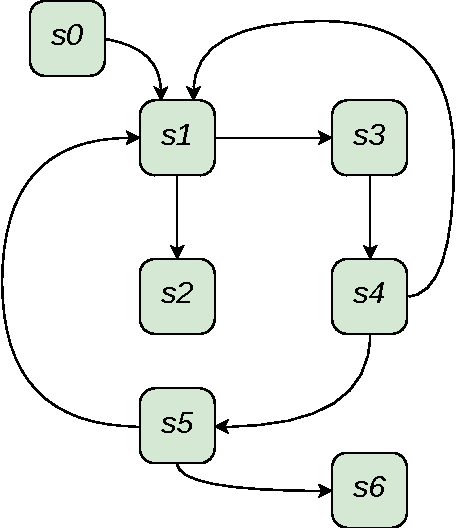
\includegraphics[width=0.8\columnwidth]{figures/SAG-Negotiation.pdf}
    \caption{Schemat algorytmu negocjacji z podziałem na stany}
    \label{fig:abstract-negotiation-fsm}
\end{figure}

Na rysunku~\ref{fig:abstract-negotiation-fsm} przedstawiony został ogólny schemat algorytmu negocjacji. W~stanie $s_{0}$ dokonywana jest inicjalizacja algorytmu. W~każdym agencie, ustawiany jest licznik rund $t$ na wartość początkową równą $1$ oraz zbiór propozycji przedstawionych $T_{i}$ jako zbiór pusty. Następnie, każdy z~agentów ustawiany jest w~stan \textit{Active} oraz przeliczany jest zbiór $b_{p_{i}}$. Ostatnim krokiem jest niedeterministyczny wybór pierwszej propozycji $\sigma$.

Po inicjalizacji, algorytm przechodzi w~stan $s_{1}$, w~którym każdy aktywny agent wykłada na stół swoją propozycję $\sigma$, równocześnie dołączając ją do swojego zbioru propozycji przedstawionych $T_{i}$. Następnie, agenci rozmawiając ze sobą szukają takiej propozycji, która odpowiada wszystkim aktywnym agentom. Jeżeli taka propozycja zostanie znaleziona, następuje przejście do stanu terminalnego $s_{2}$. W~przeciwnym przypadku, należy znaleźć agenta, który powinien odpuścić w~danej rundzie negocjacji. Aby znaleźć takiego agenta, negocjacje przechodzą do stanu $s_{3}$.

W~stanie $s_{3}$, każdy z~aktywnych agentów oblicza swoje ryzyko. Ryzyko jest liczbową wartością jak dużo agent może stracić, innymi słowami jak bardzo może wzrosnąć koszt agenta jeżeli w~danej rundzie odpuści. Z~wszystkich agentów, wybierani jest zbiór agentów $g$, dla których ryzyko jest najmniejsze. Po określeniu zbioru $g$, negocjacje przechodzą do stanu $s_{4}$.

W~stanie $s_{4}$ następuje etap szukania kompromisu. Propozycję kompromisową zaproponować mogą tylko agenci ze zbioru $g$, określonego w~poprzednim kroku. Agenci poszukują \emph{prawdziwego kompromisu}, czyli takiej propozycji która jest co najmniej tak dobra dla każdego agenta jak ta którą zaproponował w~danej rundzie oraz lepsza dla co najmniej jednego innego agenta. Proponowane rozwiązanie nie może zwiększać kosztu globalnego całej fabryki oraz nie może być już wcześniej zaproponowane przez agenta szukającego kompromisu. Jeżeli agent znajdzie propozycję spełniającą podane obostrzenia, to zaproponuje ją w~następnej rundzie negocjacji. Negocjacje przechodzą do stanu $s_{1}$ i~rozpoczyna się kolejna iteracja. Jeżeli nie to agent przechodzi do stanu $s_{5}$.

Obostrzenia dotyczące \emph{prawdziwego kompromisu} są dosyć spore, dlatego też może zdarzyć się że agent nie znajdzie takiej sekwencji. W~takim przypadku, w~stanie $s_{5}$ agent ponownie przelicza swój zbiór propozycji $b_{p_{i}}$. Jeżeli jest on niepusty, to w~następnej iteracji zaproponuje jedną z~sekwencji z~nowego zbioru $b_{p_{i}}$, wybraną w~sposób niedeterministyczny.

Może dojść do sytuacji że nowy zbiór $b_{p_{i}}$ będzie zbiorem pustym, co świadczy o~wyczerpaniu możliwych propozycji. W~takim przypadku, agent przechodzi w~stan nieaktywny i opuszcza stół negocjacyjny. Na rysunku~\ref{fig:abstract-negotiation-fsm} zostało to przedstawione jako przejście do stanu $s_{6}$. Przejście do tego stanu znaczy że agent wyczerpał swoje możliwości negocjacyjne i~zgadza się na wszystkie inne propozycje, przedstawione w~dalszych etapach.
